\section{Nota Teórica}
\subsection{Microcontrolador STM32F429}
\subsubsection{Características Generales}
El microcontrolador STM32F429ZIT6 es una unidad potente y versátil basada en el núcleo ARM 32-bits Cortex-M4 con FPU (unidad de punto flotante). Esta unidad RISC opera a una frecuencia de hasta 180 MHz.

\subsubsection{Memoria y Almacenamiento}
El STM32F429ZIT6 posee una memoria flash de 2 MB y una SRAM de 256 KB. Además, cuenta con un SDRAM adicional de 64-Mbit.


\subsubsection{Comunicación y Conectividad}
\begin{itemize}
    \item USB OTG con conector Micro-AB.
    \item Seis LEDs para diferentes propósitos, incluidos USB Comms y Power On.
    \item Dos push-buttons (Usuario y reset).
    \item Header para LQFP144 I/Os.
    \item Funciones USB: Debug, virtual COM y almacenamiento.
    \item 21 interfaces de comunicaciones que incluyen I2C, USART, SPI, SAI y CAN.
    \item Conectividad avanzada USB 2.0.
    \item Sensor de movimiento I3G4250D y giroscopio STM EMS de 3-ejes.
\end{itemize}

\subsubsection{Alimentación y Energía}
El microcontrolador puede ser alimentado a través de USB o una fuente externa de 3V o 5V. Posee características de bajo consumo para aplicaciones de bajo poder.

\subsubsection{Otras Características}
\begin{itemize}
    \item Controlador LCD-TFT.
    \item 3 ADCs de 12-bit.
    \item 2 convertidores D/A de 12-bit.
    \item 17 timers: 12 de 16-bit y 2 de 32-bit que operan a hasta 180 MHz.
    \item Capacidades de debug: SWD y JTAG.
    \item 168 I/Os con capacidad de interrupción.
    \item Interfaz de cámara.
    \item True RNG (generador de números aleatorios).
    \item CRC (verificación de redundancia cíclica).
    \item Controladores DMA.
\end{itemize}
\subsubsection{Diagrama de bloques}
\begin{figure}[H]
    \centering
    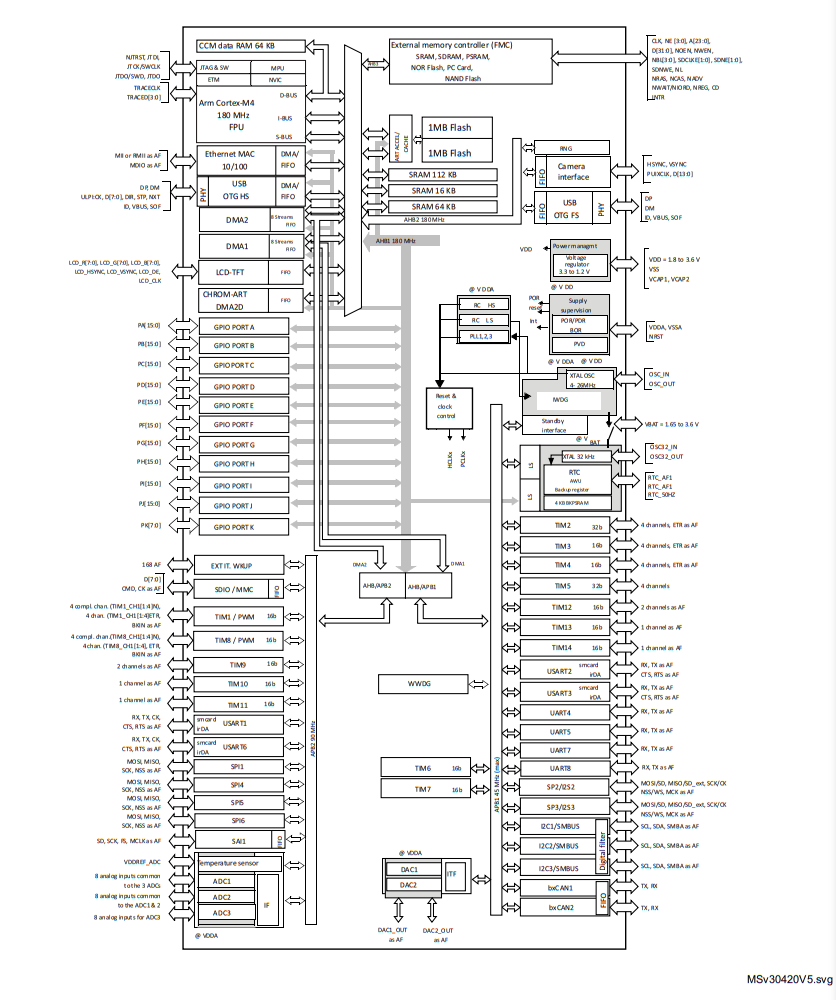
\includegraphics[scale=0.8]{images/Diagrama_bloques.png}
    \caption{Diagrama de bloques. \cite{STM32F429xxDatasheet}}
    \label{fig:bloques}
\end{figure}
\subsubsection{Características eléctricas}
\begin{figure}[H]
    \centering
    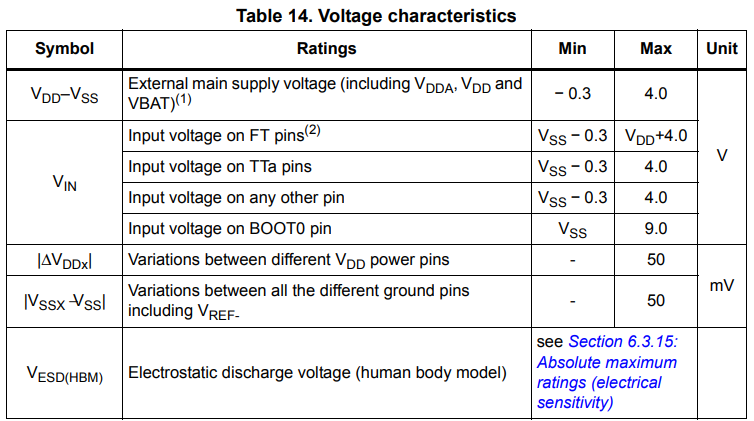
\includegraphics[scale=0.7]{images/Carac_Volt.png}
    \caption{Características de voltaje. \cite{STM32F429xxDatasheet}}
    \label{fig:car_vol}
\end{figure}
\begin{figure}[H]
    \centering
    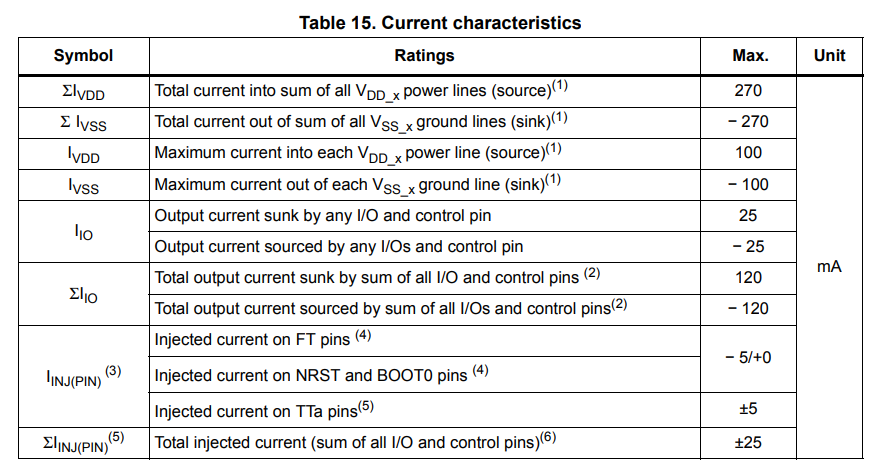
\includegraphics[scale=0.7]{images/Carac_Corr.png}
    \caption{Características de corriente. \cite{STM32F429xxDatasheet}}
    \label{fig:car_cor}
\end{figure}
\subsubsection{Diagrama de pines}
\begin{figure}[H]
    \centering
    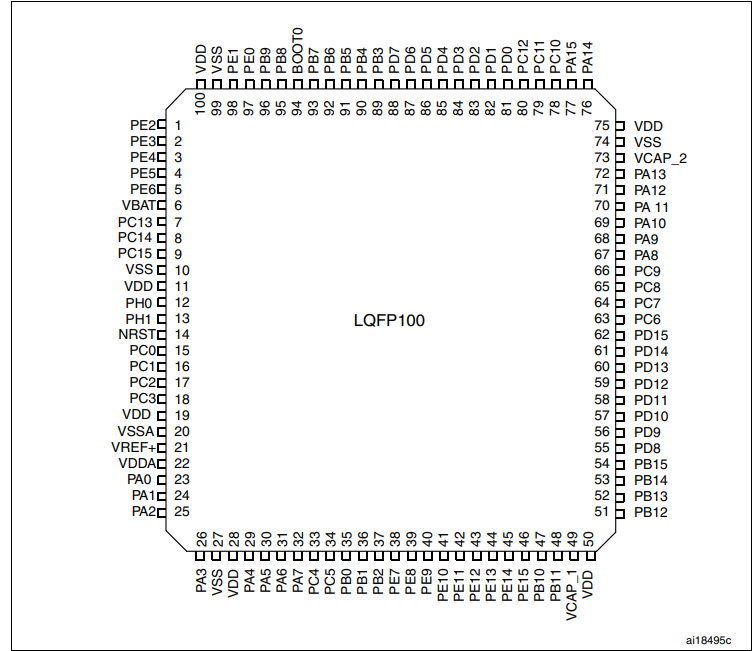
\includegraphics[scale=0.5]{images/diag_pin.png}
    \caption{Diagrama de pines. \cite{STM32F429xxDatasheet}}
    \label{fig:pines}
\end{figure}
\subsubsection{Sensor L3GD20}
El sensor \textbf{MEMS L3GD20} es un giroscopio de tres ejes desarrollado por STMicroelectronics. Este sensor es particularmente destacado por su bajo consumo y capacidad para medir la tasa angular con respecto a un entorno externo. Es decir, puede detectar movimientos de rotación a lo largo de sus tres ejes ortogonales. Para la comunicación con microcontroladores u otros dispositivos, el L3GD20 ofrece interfaces tanto I2C como SPI.

En el contexto del \textbf{STM32F429 Discovery Kit}, este sensor se comunica específicamente a través del protocolo SPI, conectado en la interfaz SPI5 del microcontrolador. La configuración y comunicación con el L3GD20 se realiza mediante instrucciones SPI. Existen varios registros esenciales para su operación:

\begin{itemize}
    \item \texttt{WHOAMI}: Un identificador único que se puede usar para validar la configuración al leer su valor.
    \item \texttt{CTRLREG1}: Se encarga del control de ejes y del modo de energía.
    \item \texttt{CTRLREG2}: Es responsable de la configuración del filtro de paso alto.
    \item \texttt{CTRLREG4}: Define la configuración de los dps y el modo SPI.
\end{itemize}

Para operar el L3GD20 con el STM32F429, es necesario realizar una serie de pasos de configuración, que incluyen habilitar el reloj para el SPI, configurar pines, inicializar y configurar el protocolo SPI y, finalmente, configurar el L3GD20 a través de la interfaz SPI.
\subsubsection{Pantalla y Gráficos}
El microcontrolador tiene un controlador LCD-TFT integrado y está equipado con una pantalla TFT LCD de 2.4" QVGA.

La \textbf{Pantalla LCD/TFT ILI9341} es una pantalla táctil a color con una resolución de 240x320 píxeles. Esta pantalla utiliza el controlador gráfico ILI9341 y un controlador táctil XPT2046 para la detección de toques. A nivel de comunicación, esta pantalla ofrece interfaces I2C y SPI, y en el contexto del \textbf{STM32F429 Discovery Kit}, se comunica específicamente a través de la interfaz SPI5. Como con otros dispositivos periféricos, la configuración y comunicación con el ILI9341 se realiza mediante instrucciones SPI.

El controlador STM32F429 incluye características específicas para el manejo de pantallas, como\cite{STM32F429xxDatasheet}:

\begin{itemize}
    \item Interfaz paralela LCD en modos 8080/6800.
    \item Controlador LCD-TFT con resolución completamente programable, capaz de manejar hasta un ancho de 4096 píxeles, una altura de 2048 líneas y un reloj de píxeles de hasta 83 MHz.
    \item Capacidades para interfaz con la mayoría de los controladores gráficos LCD, soportando los modos Intel 8080 y Motorola 6800.
    \item Controlador de pantalla LCD-TFT que proporciona una salida RGB paralela digital de 24 bits, compatible con una amplia gama de paneles LCD y TFT hasta resolución XGA (1024x768) con características como:
    \begin{itemize}
        \item Dos capas de visualización con FIFO dedicado (64x32-bit).
        \item Tabla de búsqueda de colores (CLUT) de hasta 256 colores (256x24-bit) por capa.
        \item Hasta 8 formatos de color de entrada seleccionables por capa.
        \item Fusión flexible entre dos capas usando un valor alfa (por píxel o constante).
        \item Parámetros programables flexibles para cada capa.
        \item Clave de color (color de transparencia).
        \item Hasta 4 eventos de interrupción programables.
    \end{itemize}
\end{itemize}


\newpage
\subsection{Precios de los componentes}

A continuación se muestran la lista de precios de los componentes utilizados



\begin{table}[h]
\centering
\begin{tabular}{|c|c|}
\hline
\textbf{Componente} & \textbf{Precio (Colones)} \\ \hline
    STM32F429   &  24890.09                   \\ \hline
    Resistencias $680 \Omega$   &  75                   \\ \hline
    Resistencia $3.3 K\Omega$   &  35                   \\ \hline
    Resistencia $5.1 K\Omega$   &  55                   \\ \hline
    Batería $9 V$   &  2395                   \\ \hline
    
    

\end{tabular}
\caption{Precio de los componentes}
\label{tab:my-table}
\end{table}